\documentclass[a4j]{jarticle}
\usepackage{fancybox,ascmac,amsmath,amssymb,graphicx}
\begin{document}

\section{Design of Butterworth Lowpass Filter}

\begin{itembox}[l]{{\large {\bf Butterworth Approximation}}}
1. Define specification of the filter, \( H_0 \): DC Gain, \( H_c \): Gain at cutoff frequency, \( H_s \) Gain at stopband edge frequency, \( \omega_c \): Cutoff frequency (rad/s), \( \omega_s \): Stopband frequency (rad/s). 
Also choose the optimization strategy: stopband edge frequency gain optimized or passband edge gain optimized.\\
2. Calculate normalized cutoff frequency \( \Omega_s \)
\begin{eqnarray*}
\Omega_{c} &=& 1 \\
\Omega_{s} &=& \frac{\omega_s}{\omega_c}
\end{eqnarray*}
3. Calculate \( \beta = \beta_{max} \) on stopband edge frequency gain optimized or \( \beta = \beta_{min} \) on passband edge gain optimized.
\begin{eqnarray*}
\beta_{max} = \sqrt{\left(\frac{H_0}{H_c}\right)^2-1}\\
\beta_{min} = \sqrt{\frac{\left(\frac{H_0}{H_s}\right)^2-1}{\Omega_s^2}}
\end{eqnarray*}
4. Calculate the order of the filter \( N \) by rounding up \( n_{fmin} \) to the next integer:
\begin{eqnarray*}
n_{fmin} &=& \frac{\log\left(\frac{{\frac{H_0^2}{H_s^2}-1}}{{\frac{H_0^2}{H_c^2}-1}}\right)}{2\log\Omega_s}
\end{eqnarray*}
5. Calculate \( s_{k+} \), the roots of the transfer function denominator polynomial equation:
\begin{eqnarray*}
s_{k+} &=& \sqrt[N]{\frac{1}{\beta}}\mathrm{e}^{j\left(\frac{2k+1}{2N}\pi+\frac{\pi}{2}\right)}\quad k=0,1, \cdots N-1
\end{eqnarray*}
\end{itembox}

\clearpage

{\large {\bf Example 1}} Determine the transfer function of Butterworth lowpass filter of stopband edge frequency gain optimized,
 \( H_0 \) = 1, \( H_c \) = 0.891 ( = -1dB) , \( H_s \) = 0.00398 ( = -48dB) ,
 Cutoff frequency = 125664 (=20kHz), Stopband edge frequency = 1108353 (=176.4kHz) \\

{\large {\bf 1. Perform Butterworth Approximation}}

\begin{eqnarray*}
\Omega_{c} &=& 1 \\
\Omega_{s} &=& \frac{\omega_s}{\omega_c} = 8.82 \\
n_{fmin} &=& 2.85 \\
N &=& Ceiling(2.85) = 3 \\
\beta_{max} &=& 0.509 \\
\textmc{angle of } s_k &=& \frac{2k+1}{2N}\pi + \frac{\pi}{2} \\
\textmc{magnitude of } s_k &=& \beta^{\frac{-1}{N}} \\
s_k &=& magnitude \left\{ \cos( angle ) + i\sin( angle) \right\} \\
s_0 &=& 1.25 \left\{ \cos(2.09) + i\sin(2.09) \right\} \\
s_1 &=& 1.25 \left\{ \cos(\pi) + i\sin(\pi) \right\} = -1.25\\
s_2 &=& 1.25 \left\{ \cos(4.19) + i\sin(4.19) \right\} \\
\textmc{Transfer function} H(s) &=& \frac{1}{(s-1.25 \left\{ \cos(2.09) + i\sin(2.09) \right\})(s+1.25)(s-1.25 \left\{ \cos(4.19) + i\sin(4.19) \right\})}
\end{eqnarray*}

{\large {\bf 2. Partial fraction decomposition}}
\begin{eqnarray*}
H(s) &=& \frac{1}{(s-1.25 \left\{ \cos(2.09) + i\sin(2.09) \right\})(s+1.25)(s-1.25 \left\{ \cos(4.19) + i\sin(4.19) \right\})}\\
     &=& \frac{c_1}{s-1.25 \left\{ \cos(2.09) + i\sin(2.09) \right\}} + \frac{c_2}{s+1.25} + \frac{c_3}{s-1.25 \left\{ \cos(4.19) + i\sin(4.19) \right\}}\\
c_1  &=& \frac{1}{(s+1.25)(s-1.25 \left\{ \cos(4.19) + i\sin(4.19) \right\})}, s = 1.25 \left\{ \cos(2.09) + i\sin(2.09) \right\} \\
     &=& -0.6263-0.3616i \\
c_2  &=& \frac{1}{(s-1.25 \left\{ \cos(2.09) + i\sin(2.09) \right\})(s-1.25 \left\{ \cos(4.19) + i\sin(4.19) \right\})}, s = -1.25 \\
     &=& 1.253 \\
c_3  &=& \frac{1}{(s-1.25 \left\{ \cos(2.09) + i\sin(2.09) \right\})(s+1.25)}, s = 1.25 \left\{ \cos(4.19) + i\sin(4.19) \right\} \\
     &=& -0.6263+0.3616i \\
\therefore H(s) &=& \frac{-0.6263-0.3616i}{s+0.6263-1.085i} + \frac{1.253}{s+1.253} + \frac{-0.6263+0.3616i}{s+0.6263+1.085i}
\end{eqnarray*}

\clearpage

{\large {\bf 3. Multiply conjugate complex 1st order rational polynomial to get 2nd order rational polynomial with real value coefficients}}

\begin{eqnarray*}
H(s) &=& \frac{-0.6263-0.3616i}{s+0.6263-1.085i} + \frac{1.253}{s+1.253} + \frac{-0.6263+0.3616i}{s+0.6263+1.085i} \\
     &=& \frac{1.253}{s+1.253} + \frac{-0.6263-0.3616i}{(s+0.6263-1.085i)(s+0.6263-1.085i)} \\
     &=& \frac{1.253}{s+1.253} + \frac{0.523}{s^2+1.253s+1.569}
\end{eqnarray*}


{\large {\bf 4. Create lossy integrator from 1st order rational polynomial}}

\begin{eqnarray*}
H_{s1} &=& \frac{A}{s+a} \\
\omega_c &=& 20000 * 2 * \pi = 125663 \\
R_{n0} &=& 1 \\
C_{n0} &=& \frac{a}{\omega_c * R_0} \\
R_{0}  &=& R_{n0} * 10000 = 10 (k\Omega) \quad  \textmc{(frequency scaling)}\\
C_{0}  &=& \frac{C_0}{10000} = 996 \textmc{(pF)} \quad  \textmc{(frequency scaling)} \\
\end{eqnarray*}

Bug: resulted circuit does not reflect A of the rational polynomial! \\

\begin{figure}
    \centering
    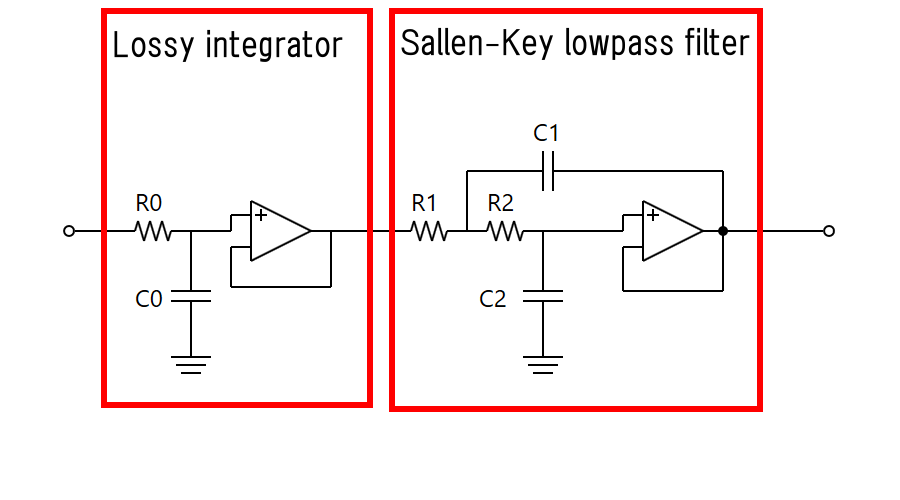
\includegraphics[width=90mm,height=50mm,natwidth=900,natheight=500]{circuit.png} \\
Figure 1
\end{figure}

{\large {\bf 5. Create Sallen-Key lowpass filter from 2nd order rational polynomial}}

\begin{eqnarray*}
H_{s2}   &=& \frac{A}{s^2+as+b} \\
\omega_0 &=& \sqrt{b} \\
\omega_c &=& 20000 * 2 * \pi = 125663 \\
Q        &=& \frac{\omega_0}{a} \\
C_{n2}   &=& 1 \\
C_{n1}   &=& \sqrt{3}*Q*C_{n2} \\
R_{n1}   &=& \frac{1}{\omega_0 * Q * C_{n2}} \\
R_{n2}   &=& \frac{1}{\sqrt(3)*\omega_0 *C_{n2}} \\
C_{1}    &=& \frac{C_{n1}}{\omega_c * 10000} = 1.38 \textmc{(nF)} \quad \textmc{(frequency scaling)} \\
C_{2}    &=& \frac{C_{n2}}{\omega_c * 10000} = 796 \textmc{(nF)} \quad \textmc{(frequency scaling)}  \\
R_{1}    &=& R_{n1} * 10000 = 7.98 (k\Omega) \quad \textmc{(frequency scaling)}  \\
R_{2}    &=& R_{n2} * 10000 = 4.61 (k\Omega) \quad \textmc{(frequency scaling)} 
\end{eqnarray*}

Bug: resulted circuit does not reflect A of the rational polynomial!

\end{document}

